\documentclass{standalone}


\usepackage{tikz}
\usepackage{pgfplots}
\usepackage{tkz-euclide}

\usetikzlibrary{positioning,calc}
\usetikzlibrary{arrows} 
\usetikzlibrary{patterns} 
\usetikzlibrary{shapes}
\usetikzlibrary{decorations.pathmorphing}
\usetkzobj{all} 
\usetikzlibrary{through}

\begin{document}



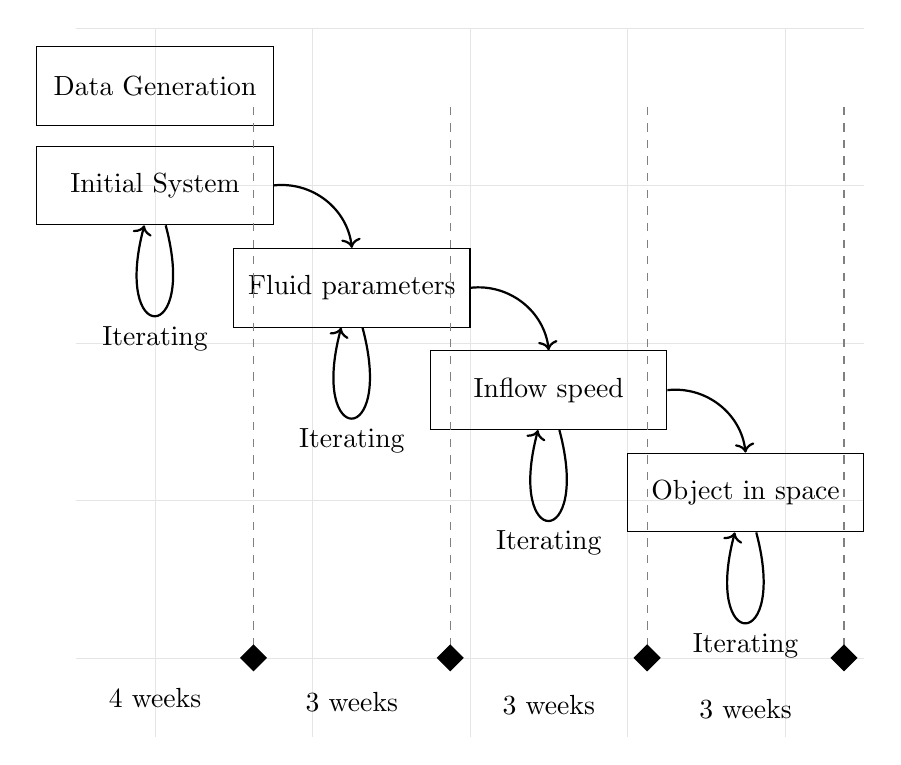
\begin{tikzpicture}
  \draw[step=2cm, gray!20!white, very thin] (-5, -3) grid (5, 6);

  \node[draw, minimum height=1cm,minimum width=3cm] at (-4, 4)     (n_1) {Initial System};
  \node[draw, minimum height=1cm,minimum width=3cm] at (-1.5, 2.7) (n_2) {Fluid parameters};
  \node[draw, minimum height=1cm,minimum width=3cm] at (1, 1.4)  (n_3) {Inflow speed};
  \node[draw, minimum height=1cm,minimum width=3cm] at (3.5, 0.1)    (n_4) {Object in space};

  \node[draw, minimum height=1cm,minimum width=3cm] [above=0.25cm of n_1] (n_0) {Data Generation};
  
  \draw [->, thick] (n_1.east) to [bend left=45] (n_2.north);
  \draw [->, thick] (n_2.east) to [bend left=45] (n_3.north);
  \draw [->, thick] (n_3.east) to [bend left=45] (n_4.north);

  \path[->,thick] (n_1) edge [loop below, looseness=15] node[text width=3cm, align=center] {Iterating} (n_1);
  \path[->,thick] (n_2) edge [loop below, looseness=15] node[text width=3cm, align=center] {Iterating} (n_2);
  \path[->,thick] (n_3) edge [loop below, looseness=15] node[text width=3cm, align=center] {Iterating} (n_3);
  \path[->,thick] (n_4) edge [loop below, looseness=15] node[text width=3cm, align=center] {Iterating} (n_4);

  
  \path[dashed, black!50!white] (-2.75, 5) edge (-2.75, -2);
  \path[dashed, black!50!white] (-0.25, 5) edge (-0.25, -2);
  \path[dashed, black!50!white] (2.25, 5) edge (2.25, -2);
  \path[dashed, black!50!white] (4.75, 5) edge (4.75, -2);

  \node [below=5.75cm of n_1] {4 weeks};
  \node [below=4.5cm of n_2] {3 weeks};
  \node [below=3.25cm of n_3] {3 weeks};
  \node [below=2.0cm of n_4] {3 weeks};

  \node at (4.75, -2)  [draw, diamond, fill=black, scale=0.7] {} ; 
  \node at (2.25, -2)  [draw, diamond, fill=black, scale=0.7] {} ; 
  \node at (-0.25, -2) [draw, diamond, fill=black, scale=0.7] {} ; 
  \node at (-2.75, -2) [draw, diamond, fill=black, scale=0.7] {} ; 

\end{tikzpicture}


\end{document}

%%% Local Variables:
%%% mode: latex
%%% TeX-master: t
%%% End:
